\documentclass[FU,HU]{matheon-poster}
% load some useful latex symbols:
\usepackage{latexsym}
% define names for even more symbols:
\usepackage{textcomp}
% define several useful macros for typesetting mathematics:
\usepackage{amsmath,amssymb}
% load mathematic fonts:
\usepackage{amsfonts}
% for typesetting paragraphs in a special form:
\usepackage{shapepar}
% for setting the examples
\usepackage{alltt}
% for extended possibilities in setting arrays and tables
\usepackage{array}
% For typesetting boxes
\usepackage[oldboxesoff]{poster-boxes}

\usepackage{color}
\usepackage{tabularx}
\usepackage{multirow}
\usepackage{enumitem}
\usepackage{tikz}

% \usepackage{epstopdf}

\newcolumntype{C}{>{\centering\arraybackslash}X}
%\newcommand{\shortitemize}{itemsep=0.25\itemsep,parsep=0.25\parsep,topsep=0.25\topsep,partopsep=0.25\partopsep}
\newenvironment{shortitemize}{\begin{itemize}[itemsep=0.25\itemsep,parsep=0.25\parsep,topsep=0.25\topsep,partopsep=0.25\partopsep]}{\end{itemize}}

% You can define colors as follows:
\definecolor{light-red}{rgb}{1, 0.59, 0.59}
\definecolor{matheonblue}{rgb}{0.0,0.2,0.4}
\definecolor{matheonlightblue}{rgb}{0.15,0.35,0.55}
\definecolor{matheonlightestblue}{rgb}{0.48,0.7,1.000}
\definecolor{matheondomainblue}{rgb}{0.0,0.2,0.4}
\definecolor{matheondarkgray}{rgb}{0.85,0.85,0.85}
\definecolor{matheonlightgray}{rgb}{0.94,0.94,0.94}
\definecolor{darkpastelgreen}{rgb}{0.01, 0.75, 0.24}
\definecolor{DarkSlateGray}{rgb}{0.184314,0.309804,0.309804}
\definecolor{color0}{rgb}{0.250980392156863,0.749019607843137,1} 
\definecolor{color1}{rgb}{0.501960784313725,0.498039215686275,1} 
\definecolor{color2}{rgb}{0.752941176470588,0.247058823529412,1}


\newcommand{\leftcolspace}{0.025\contentswidth}
\newcommand{\leftcolwidth}{0.6\contentswidth}
\newcommand{\rightcolspace}{0.65\contentswidth}
\newcommand{\rightcolwidth}{0.325\contentswidth}
\newcommand{\contwidth}{0.95\contentswidth}
    



% Define box and box title style
\tikzstyle{mybox} = [draw=matheonblue, fill=white, very thick,
    rectangle, rounded corners, inner sep=10pt, inner ysep=20pt]
\tikzstyle{fancytitle} =[fill=matheonblue, text=white, rounded corners]
    
    
\definecolor{question}{rgb}{0.29,0.29,0.73}

%Mathcal
\newcommand{\T}{\mathcal{T}}
\newcommand{\E}{\mathcal{E}}
\newcommand{\K}{\mathcal{K}}
\newcommand{\M}{\mathcal{M}}
\newcommand{\I}{\mathcal{I}}
\newcommand{\J}{\mathcal{J}}
\newcommand{\C}{\mathcal{C}}
\newcommand{\A}{\mathcal{A}}

%Mathbb
\newcommand{\R}{\mathbb{R}}
\newcommand{\N}{\mathbb{N}}

\DeclareMathOperator{\res}{Res}
\DeclareMathOperator{\osc}{osc}
\renewcommand{\div}{\textrm{div}}
\newcommand{\Jump}[1]{\lbrack #1 \rbrack \!\cdot\! \nu_E}
\newcommand{\jump}[1]{\lbrack #1 \rbrack}

\newcommand{\bnorm}[1]{\lVert #1 \rVert}
\newcommand{\anorm}[1]{\lvert\!\lvert\!\lvert#1 \rvert\!\rvert\!\rvert}
\newcommand{\norm}[2]{\lVert #1 \rVert_{#2}}
\newcommand{\Norm}[2]{\big\lVert #1\big\rVert_{#2}}
\newcommand{\snorm}[2]{\lvert #1 \rvert_{#2}}
\newcommand{\abs}[1]{\lvert #1 \rvert}

\newcommand{\hmax}{\norm{h_\ell}{L^\infty(\Omega)}}


\makeatletter
  \newcommand\huuge{\@setfontsize\huuge{18.5pt}{20}}
\makeatother

%---------------------------------------------------------------------------
\begin{document}
\titlebox {}
{\textit{International Conference On Preconditioning Techniques 2017}}
{\LARGE{Preconditioning the elastic wave equation in \\2D and 3D based on inexact MSSS matrix computations}}
{\underline{Manuel Baumann} \quad \underline{Yue Qiu} \quad Martin B. van Gijzen \hfill \small{July 31, 2017}}


\begin{pspicture}(0,0)(\contentswidth,\contentsheight)


\rput[tl](\leftcolspace,233mm){
  \posterroundedtabshadowbox{white}{\fbsdefault}{\leftcolwidth}{\large Problem statement}{
    \small\raggedright
    \vspace{0.05cm}
    
  	The discretized \textbf{time-harmonic elastic wave equation} yields,
  	\abovedisplayskip=1mm
  	\belowdisplayskip=0.5mm
	\begin{align}
	\label{eq:prob}
	(K + i {\color{matheonlightblue}\omega_k}C - {\color{matheonlightblue}\omega_k^2}M) x_k = b, \quad k = 1,...,N,
	\end{align}
	where $\{ {\color{matheonlightblue}\omega_1},...,{\color{matheonlightblue}\omega_N}\}$ are a range of (angular) frequencies.
	\begin{enumerate}
	 \item Linearization:
	 \abovedisplayskip=0.3mm
  	 \belowdisplayskip=0.3mm
	 \begin{align*}
% 	    \label{eq:lin}
	    (\mathcal{K} - {\color{matheonlightblue}\omega_k} \mathcal{M}) \mathbf{x}_k := \left\{\begin{bmatrix} i C & K \\ I & 0\end{bmatrix} - {\color{matheonlightblue}\omega_k} \begin{bmatrix} M & 0 \\ 0 & I\end{bmatrix} \right\} \begin{bmatrix} \omega_k x_k \\ x_k\end{bmatrix} = \begin{bmatrix} b \\ 0\end{bmatrix}
	\end{align*}
	 \item Apply shift-and-invert preconditioner:
	 \abovedisplayskip=0.8mm
  	 \belowdisplayskip=0.3mm
	    \begin{align}
	\mathcal{P}({\color{green!70!black}\tau})^{-1} := (\mathcal{K} - {\color{green!70!black}\tau} \mathcal{M})^{-1} \hspace{0.7cm} \text{ [cf. Fig. 3 for choice of } {\color{green!70!black}\tau} \text{]} 
	\end{align}
	\end{enumerate}
	\vspace{-0.4cm}
  }
}


\rput[tl](\leftcolspace,98.5mm){
 \posterroundedtabshadowbox{white}{\fbsdefault}{\leftcolwidth}{\large Simulation results for 2D and 3D}{
      \small\raggedright
%         \rnode{c}{
        \begin{tikzpicture}
        \node at (-1.3,5.1) {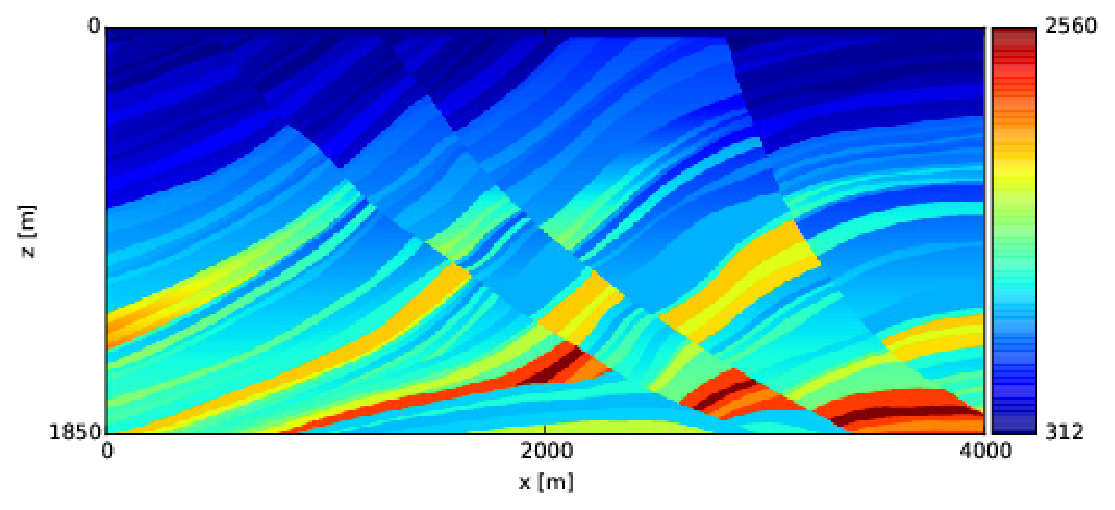
\includegraphics[scale=0.24]{cs-crop2}};
        \node at (-1.3,2.9) {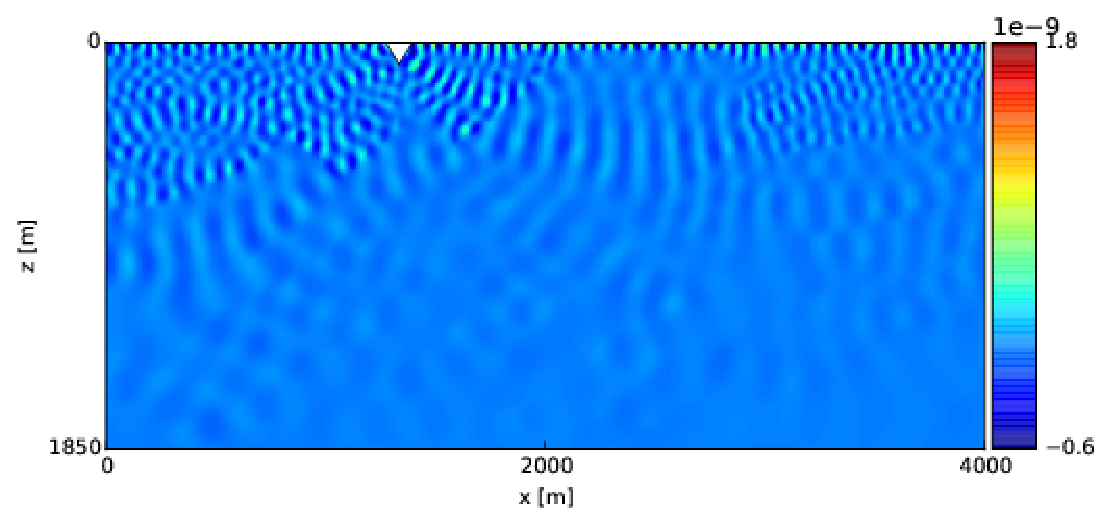
\includegraphics[scale=0.24]{disp_z10_f6-crop2}};
        \node at (3.3,4.1) {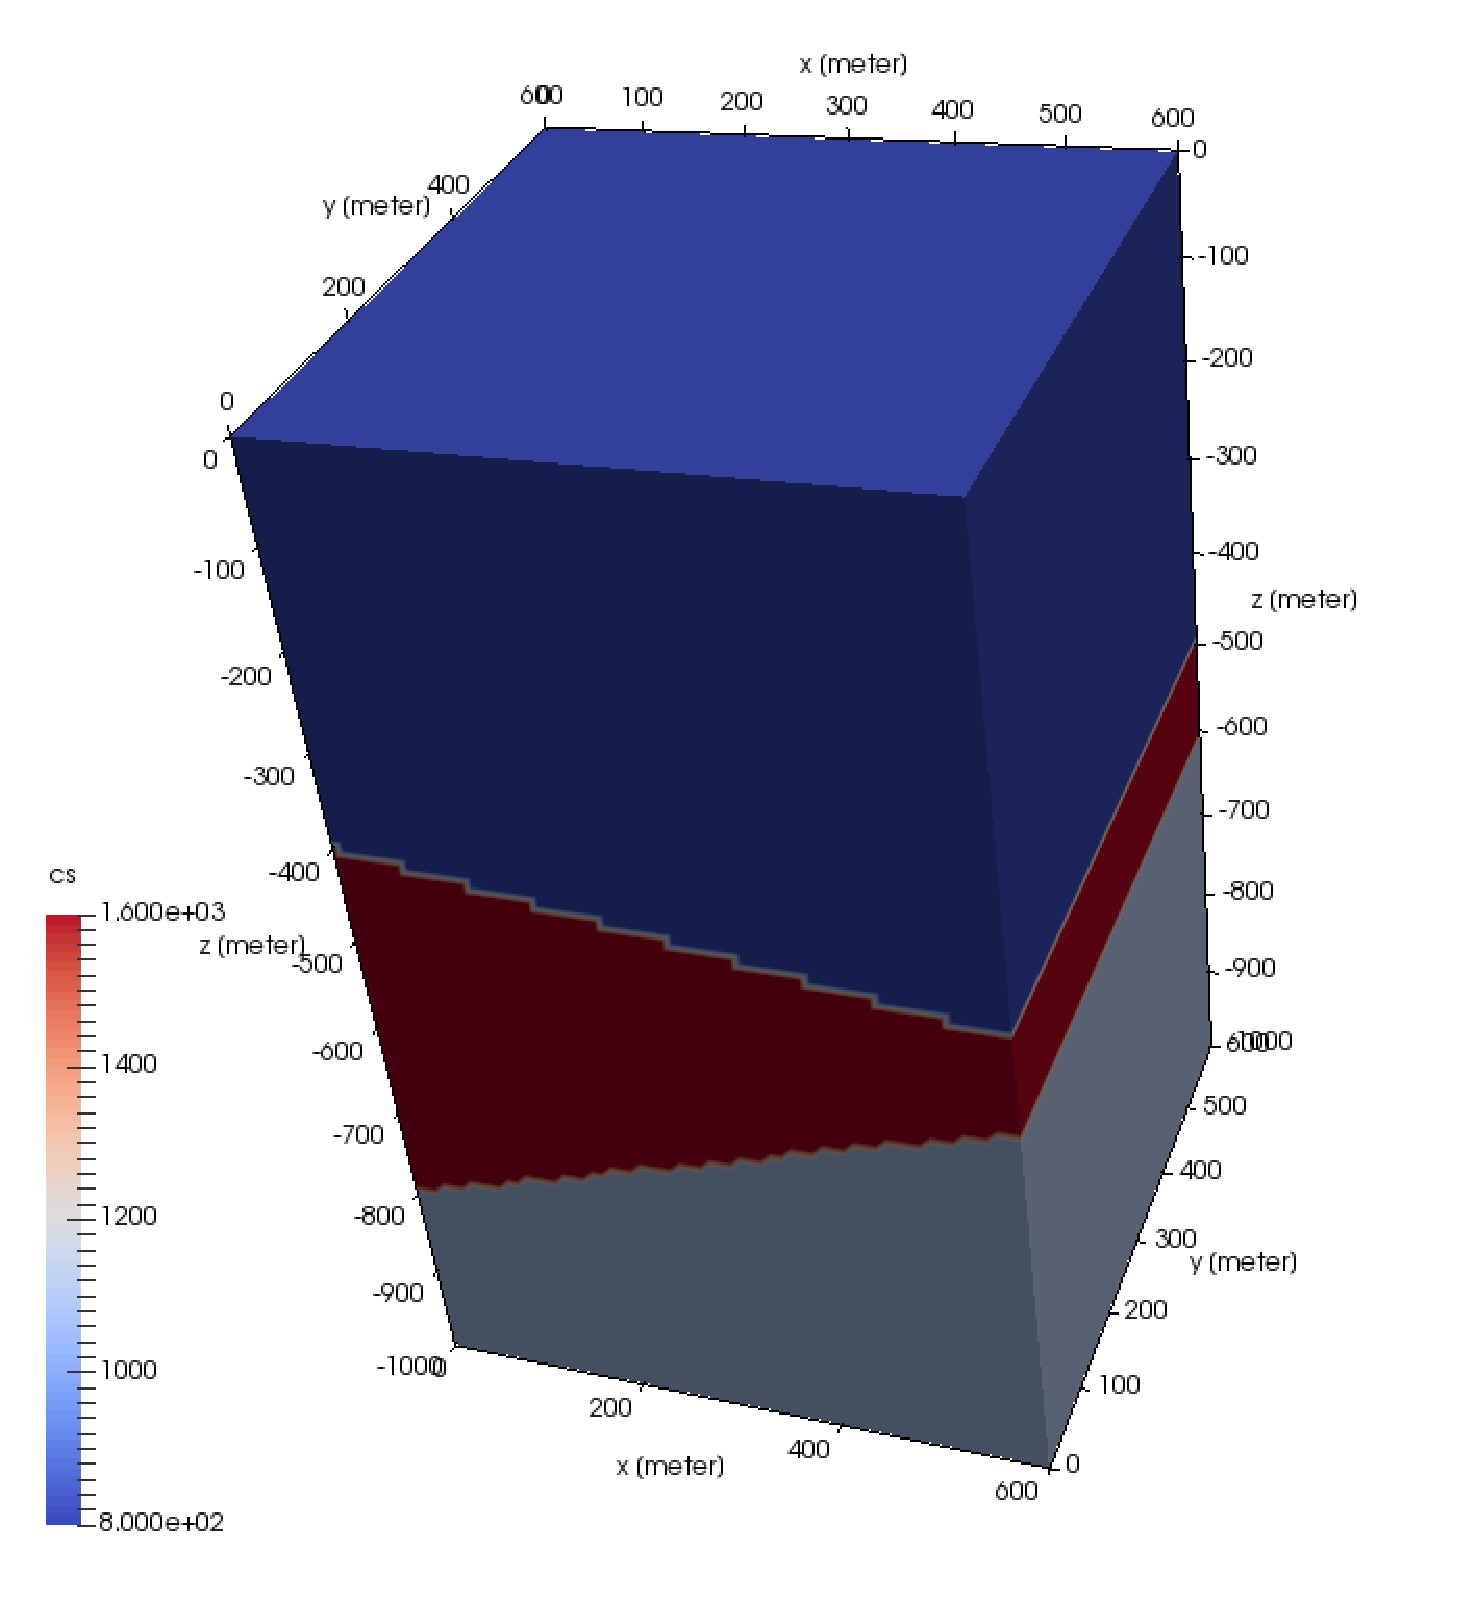
\includegraphics[scale=0.14]{wedge3d_cs}};
        \node at (6.3,4.1) {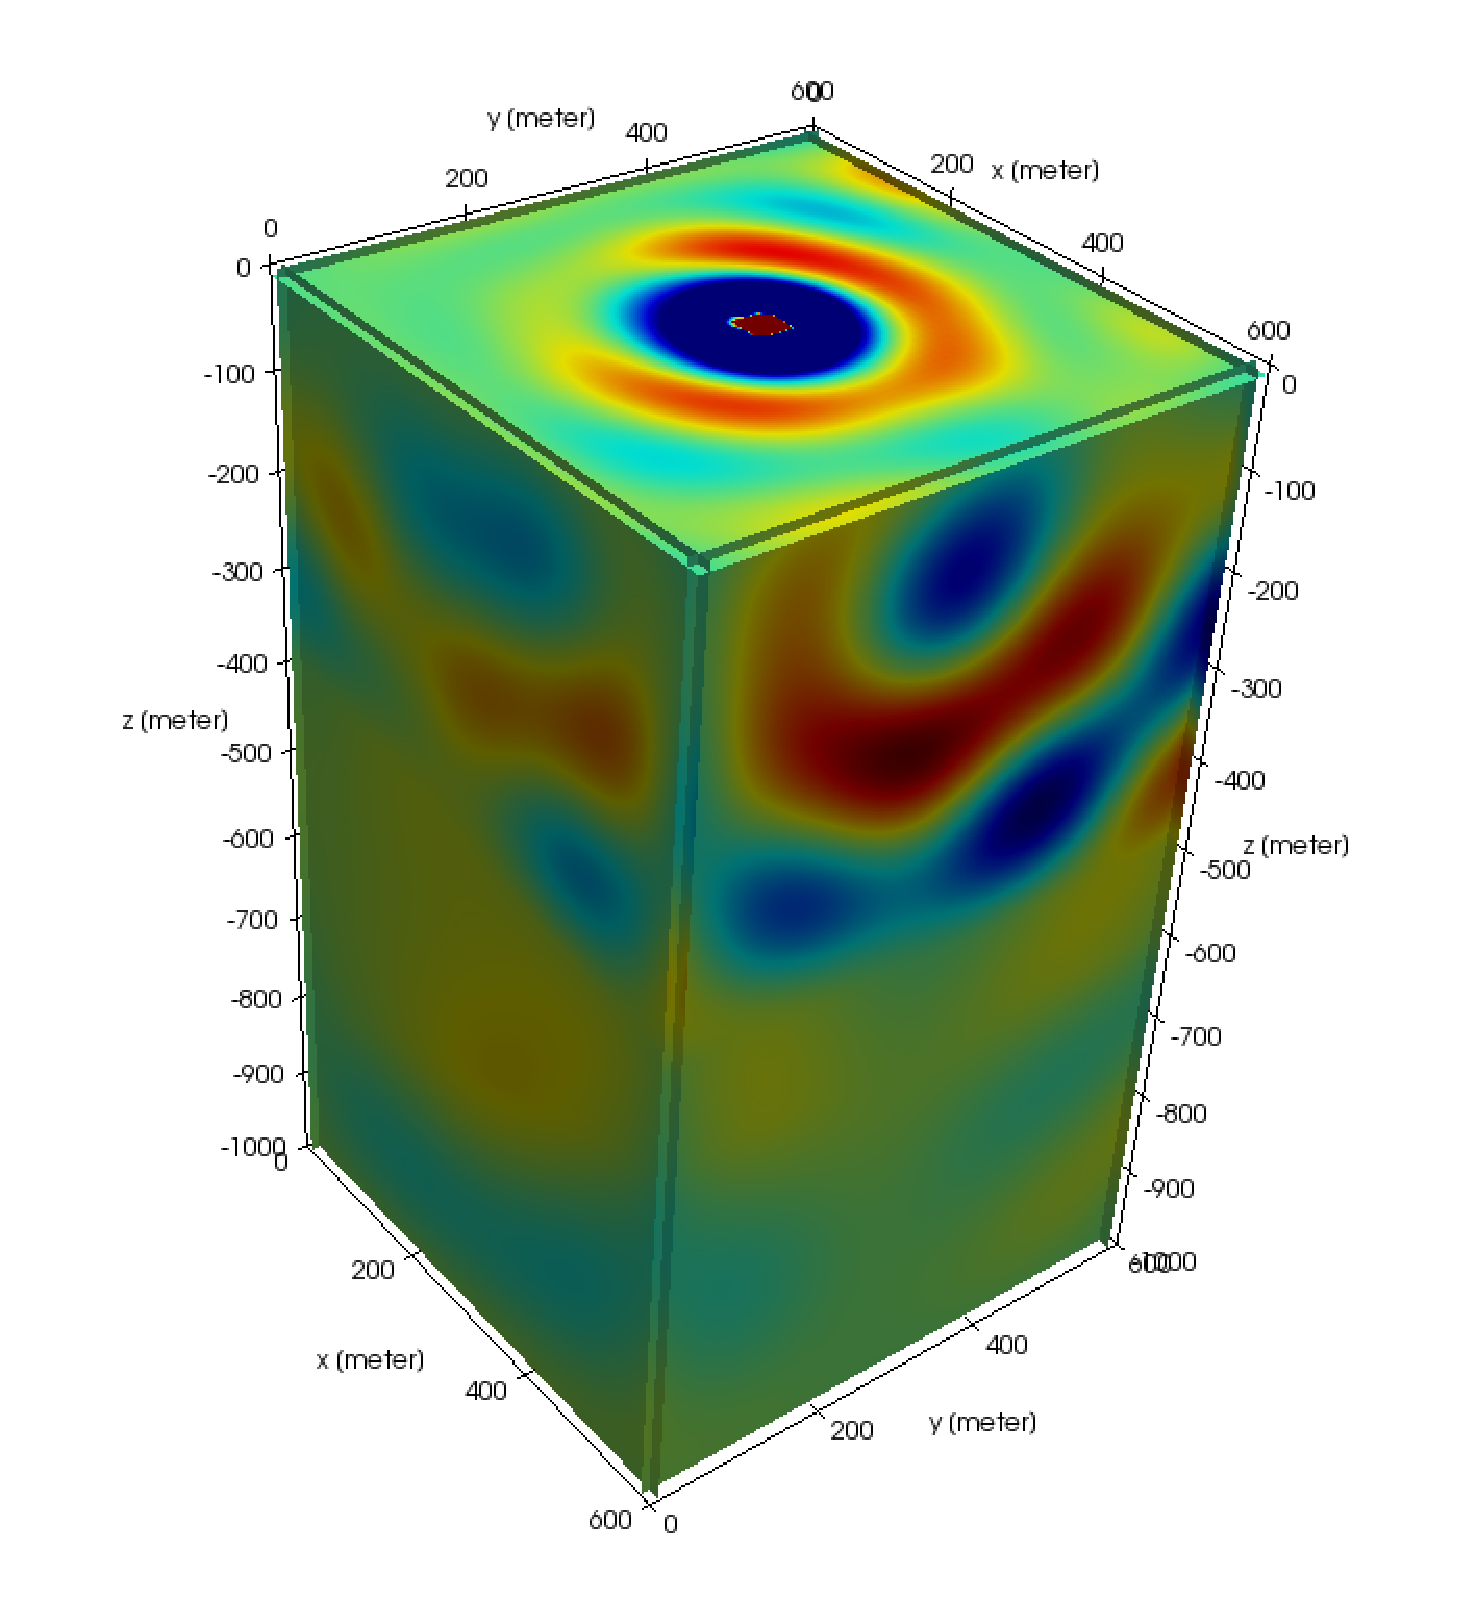
\includegraphics[scale=0.14]{wedge3d_f4}};
        \end{tikzpicture}
% 	}
	\vspace{-0.1cm}
	\centerline{Fig. 4: Simulation results for the 2D \texttt{Marmousi-II} problem, and a 3D \texttt{wedge} problem}
	
    }
    \vspace{-0.1cm}
	
}


\rput[tl](\leftcolspace,181mm){
  \posterroundedtabshadowbox{white}{\fbsdefault}{\leftcolwidth}{\large Preconditioning the elastic operator in 2D and 3D}{
     \small\raggedright
    
    For the \textbf{2D operator} (red in Fig. 2) we compute a block-LU factorization of the form $\mathcal{P}(\tau)=LSU$, with 
    \abovedisplayskip=0.8mm
    \belowdisplayskip=0.4mm
    \begin{equation*}
      L_{i,j}=\begin{cases}
             I &\hspace{-0.2cm} \text{if}\ i=j \\
             P_{i,j}{\color{magenta}S_j}^{-1} &\hspace{-0.2cm} \text{if}\ i = j+1
	     \end{cases}, \quad
      U_{i,j}=\begin{cases}
             I &\hspace{-0.2cm} \text{if}\ j=i \\
             {\color{magenta}S_i}^{-1}P_{i,j} &\hspace{-0.2cm} \text{if}\ j = i+1
	     \end{cases},     
    \end{equation*}
    and Schur complements given by
    \abovedisplayskip=0.8mm
    \belowdisplayskip=0.4mm
    \begin{equation*}
        {\color{magenta}S_i}=\begin{cases}
             P_{i,i} & \text{if}\ i=1 \\
             P_{i,i}-P_{i,i-1}{\color{magenta}S_{i-1}}^{-1}P_{i-1,i} & \text{if}\ 2\leq i\leq n_x.
	     \end{cases}
    \end{equation*}
    Here, the matrices {\color{magenta}$S_i$ are SSS} matrices, and inverses are computeted inexactly.
    
    \vspace{0.5cm}
    
    For the \textbf{3D operator}, we consider
    \abovedisplayskip=0.8mm
    \belowdisplayskip=0.3mm
     \begin{align*}
  \mathcal{P}_h(\tau) %&= {\color{orange}P_\text{SSOR}^{-1}} + {\color{matheonblue}P_\text{CGC}} \\
                           = \underbrace{{\color{orange}(LD^{-1}+I)D(D^{-1}U+I)}}_{\text{''}n_z \text{ times a 2D problem``}} +  \underbrace{{\color{matheonblue}P \mathcal{P}_H(\tau)^{-1} R}}_{\text{''small 3D``}}
 \end{align*}
    \begin{itemize}
    \item The {\color{orange}block SSOR} preconditioner makes use of efficient 2D computations.
    \item Additive {\color{matheonblue}coarse grid correction} yields grid-independent convergence.
%     \item
    \end{itemize}
    
}}

% \rput[tl](\leftcolspace,181mm){
%   \posterroundedtabshadowbox{white}{\fbsdefault}{\leftcolwidth}{\large Preconditioning multi-shift wave propagation problems }{
%      \small\raggedright
%     \begin{tikzpicture}[overlay]
%      \node at (9.5,-0.32) {${\color{gray}\mathcal{A} := \begin{bmatrix} i C & K \\ I & 0\end{bmatrix},\ \mathcal{B} := \begin{bmatrix} M & 0 \\0 & I\end{bmatrix}}$};
%     \end{tikzpicture}
%     
%     \vspace{0.05cm}
%        	Right-preconditioning of \eqref{eq:lin} yields,
%        	 \belowdisplayskip=0.9mm
%        	\begin{align*}
% (\mathcal{A}-\omega_k\mathcal{B})\mathcal{P}_k^{-1}\mathbf{y}_k = \mathbf{b} \quad \Leftrightarrow \quad  (\mathcal{A}(\mathcal{A}-{\color{red}\tau} \mathcal{B})^{-1}  - \eta_k I) \mathbf{y}_k = \mathbf{b},
% \end{align*}
% where $\eta_k = \omega_k/(\omega_k-{\color{red}\tau})$ and $\mathcal{P}_k = (1-\eta_k) (\mathcal{A}-{\color{red}\tau} \mathcal{B})$.
% \begin{itemize}
%  \item Use \textsf{MSSS} matrix computations to approximately apply $(\mathcal{A}- {\color{red}\tau} \mathcal{B})^{-1}$, cf. Figure 2.
%  \item Choose ${\color{red}\tau}$ optimally in the sense of,
%         \abovedisplayskip=0.8mm
%         \belowdisplayskip=0.3mm
% 	\begin{align*}
% 	\tau^\ast = \min_{\tau \in \mathbb{C}} \max_{k=1,...,N} \left( \frac{R_{\color{gray}k}(\tau)}{|c_k(\tau)|} \right), \quad \text{cf. Figure 3.}
% 	\end{align*}
% 
% \end{itemize}
% 
% \begin{tikzpicture}
% \node [mybox] (box){%
%     \begin{minipage}{0.93\textwidth}
%     \vspace{-0.4cm}
%     Let the eigenvalues of the preconditioned matrix be enclosed by a circle of radius $R$ and center $c$. Then the GMRES-residual norm after $i$ iterations $\|r^i\|$ satisfies,
%     \abovedisplayskip=0.5mm
%     \belowdisplayshortskip=0.1mm
%     \begin{align*}
%     \frac{\|r^i\|}{\|r^0\|} \leq c_2(X) \left( \frac{R}{|c|} \right)^i,
%     \end{align*}
%     where $X$ is the matrix of eigenvectors, and $c_2(X)$ its condition number in $2$-norm.
%     \vspace{-0.5cm}
%     \end{minipage}
% };
% \node[fancytitle, right=10pt] at (box.north west) {Theorem: GMRES convergence bound [Y. Saad, 2003]};
% \end{tikzpicture}%
% \vspace{-0.2cm}
% }}


\rput[tl](\rightcolspace,233mm){
  \posterroundedshadowbox{white}{3.5mm}{\rightcolwidth}{
    \small\raggedright \rnode{c}{
	\hspace{0.1cm}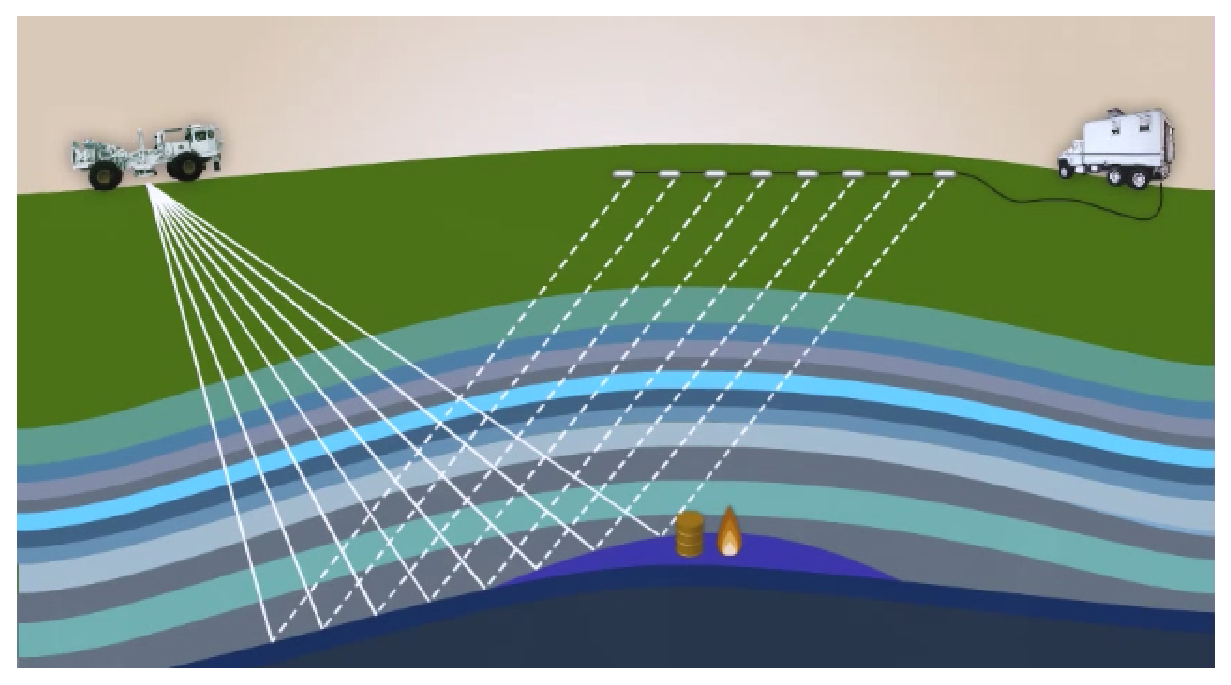
\includegraphics[scale=0.27]{Seismic}
	}
	\vspace{0.1cm}{
	\centerline{Fig. 1: Full-waveform inversion}}
	\begin{tikzpicture}[overlay]
	 \node at (4.4,1.05) {\footnotesize{{\color{white}\copyright \ geophysicsRocks!}}};
	\end{tikzpicture}
        \vspace{-0.3cm}
	}
}


\rput[tl](\rightcolspace,179mm){
  \posterroundedtabshadowbox{white}{\fbsdefault}{\rightcolwidth}{\large MSSS matrix structure}{
    \small\raggedright
    \vspace{0.1cm}
    \rnode{c}{
    \hspace{-0.25cm}
      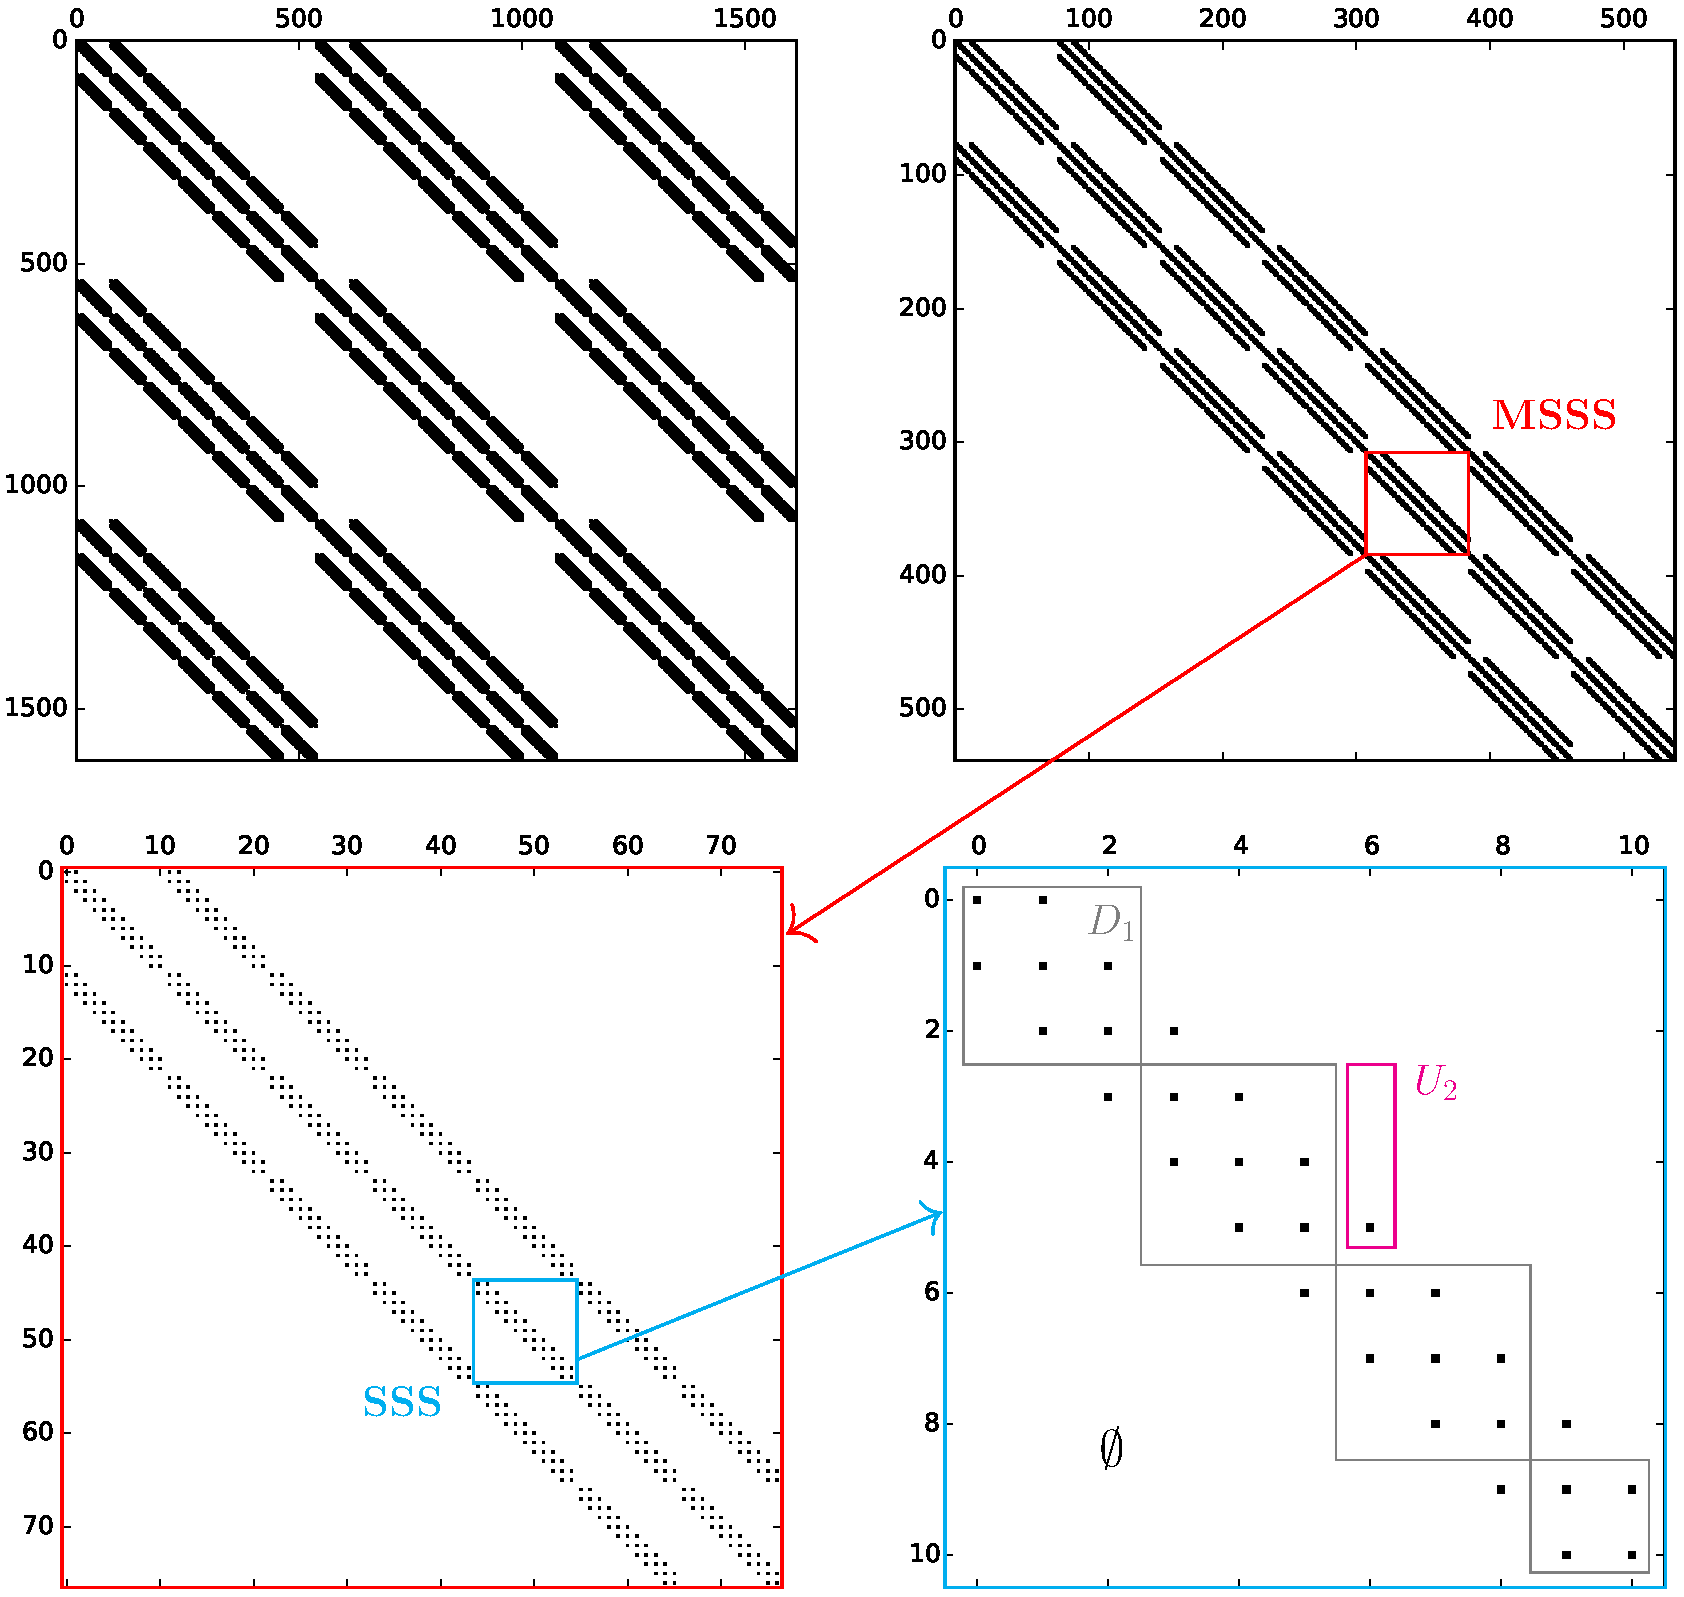
\includegraphics[scale=0.2]{3d_hier_matrix}}
	\vspace{-0.3cm}{
	\centerline{Fig. 2: \textsf{MSSS} structure of the 3D matrix \eqref{eq:prob}}}
}}

\rput[tl](\rightcolspace,97.7mm){
  \posterroundedtabshadowbox{white}{\fbsdefault}{\rightcolwidth}{\large Preconditioned spectra}{
    \small\raggedright 
\vspace{0.2cm}
    \rnode{c}{
    \hspace{0.2cm}
      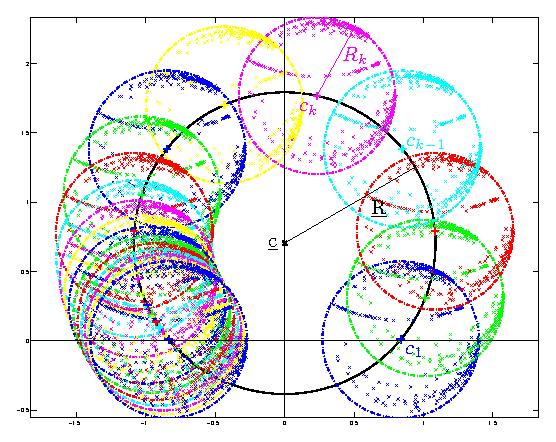
\includegraphics[scale=0.55]{spec_pic}
      }
      \vspace{0.3cm}
	\vspace{-0.2cm}{
	\centerline{Fig. 3: Spectra after M\"obius transformation}}
}}

\rput[tl](17.1cm,33mm){
  \posterroundedshadowbox{white}{1.5mm}{3.3cm}{
	\centering
% 	
\includegraphics[scale=0.34]{qrcode}
	
\includegraphics[scale=0.165]{qr_paper}
	}
}


\rput[tl](\leftcolspace,33mm){
  \posterroundedtabshadowbox{white}{\fbsdefault}{16cm}{\large References}{
  \renewcommand\refname{\vskip -0.4cm}
  \begin{thebibliography}{10}
  \footnotesize \setlength{\parskip}{0cm}
%   \bibitem{1}
%   M. Baumann and M.B. van Gijzen (2017).
%   \newblock {\em  An Efficient Two-Level Preconditioner for Multi-Frequency Wave Propagation Problems.}
%   \newblock DIAM Technical Report \textbf{17-03}, TU Delft.
  \bibitem{0}
  M. Baumann, R. Astudillo, Y. Qiu, E.Y.M. Ang, M.B. van Gijzen, and R.-E. Plessix (2017).
  \newblock {\em An MSSS-Preconditioned Matrix Equation Approach for the Time-Harmonic Elastic Wave Equation at Multiple Frequencies.}
  \newblock Springer Computat. Geosci., DOI: 10.1007/s10596-017-9667-7.
%    \bibitem{2}
%    M. Baumann and M.B. van Gijzen (2015).
%    \newblock {\em Nested Krylov methods for shifted linear systems.}
%    \newblock SIAM Journal of Scientific Computing, \textbf{37}(5), S90-S112.
  \bibitem{3}
  Y. Qiu (2015). 
  \newblock {\em Preconditioning Optimal Flow Control Problems Using Multilevel Sequentially Semiseparable Matrix Computations.}
  \newblock PhD Thesis, Delft University of Technology.
  \end{thebibliography}
  \vspace{-0.6cm}
  }
}

\end{pspicture}
\end{document}
